\documentclass[final,hyperref={pdfpagelabels=false}, professionalmath, mathserif, 11pt]{beamer}
\usepackage{grffile}
\mode<presentation>{\usetheme{BGC_retreat}}
\usepackage[english]{babel}
\usepackage[utf8]{inputenc}
\usepackage{graphicx}

 
\def\mytitle{Radiocarbon and the transit time of carbon in terrestrial ecosystems }
%\def\mysubtitle{Application to Stability}
\def\myauthor{Carlos A. Sierra  \quad Markus Müller}
\def\myfooter{

\includegraphics[height=7ex]{qrcode.png}
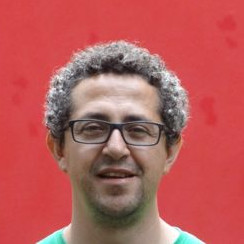
\includegraphics[height=7ex]{Sierra.jpg}
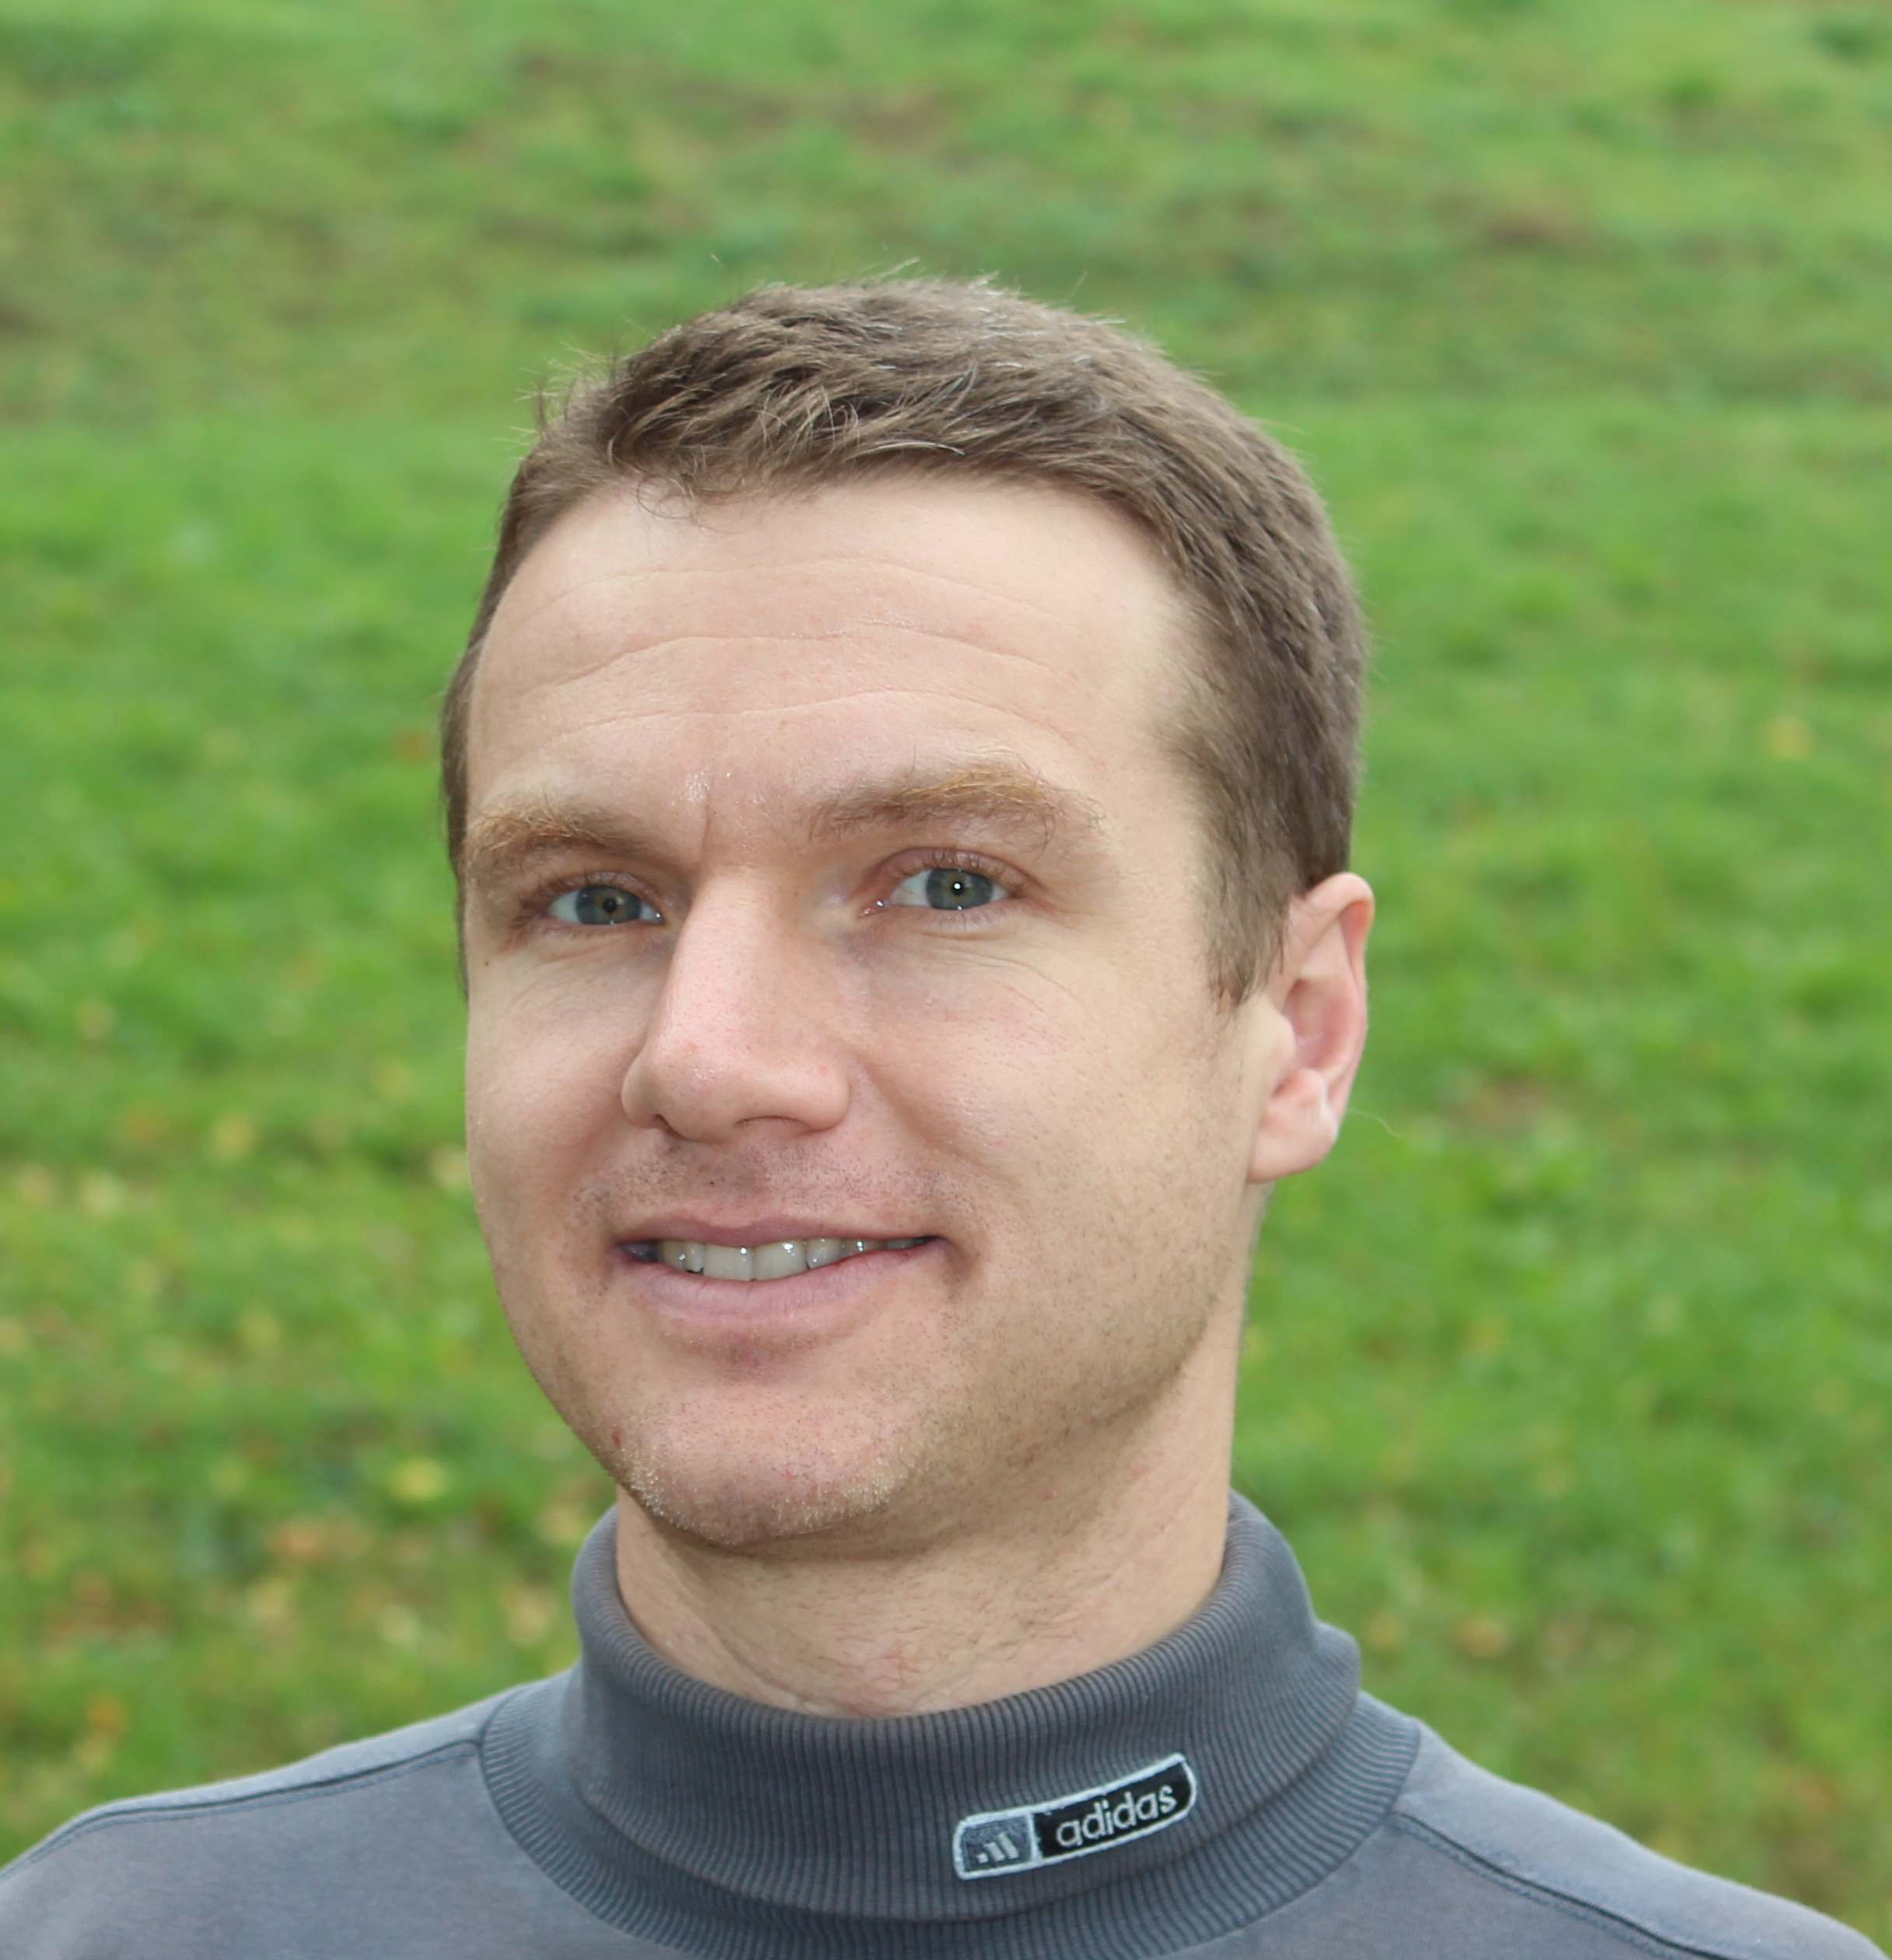
\includegraphics[height=7ex]{MarkusMueller.jpg}
}

\usepackage{setspace}
\setstretch{1.25}

\usepackage{bm}
\usepackage{tikz}
\usetikzlibrary{arrows,backgrounds,calc,chains,fadings,fit,graphs,mindmap,patterns,positioning,quotes,scopes,shapes.geometric,trees} 

\definecolor{yellow}{rgb}{1,1,0}
\definecolor{green}{rgb}{0,1,0}
\definecolor{GeneralModel}{rgb}{0.709803921568627,0.870588235294118,0.63921568627451}
\definecolor{TheoreticalAnalysis}{rgb}{1,1,0.8}
\definecolor{SoilPy}{rgb}{0.63921568627451,0.83921568627451,0.8}
\definecolor{SoilR}{rgb}{0.8,0.8,1}

\colorlet{lightblue}{blue!25}
\colorlet{darkblue}{blue!75}
\colorlet{lightpink}{red!12}
\colorlet{darkred}{red!75}
\colorlet{red}{red!50}
\colorlet{LTICTBg}{lightpink}
\colorlet{GASDSTBg}{blue}
\colorlet{LDSTBg}{yellow!30!blue!30}

%%%%<
%\usepackage{verbatim}
%\usepackage[active,tightpage]{preview}
%\PreviewEnvironment{tikzpicture}
%\setlength\PreviewBorder{5pt}%
%%%%>

%node[pos=0.5]{yes}
\DeclareRobustCommand{\intl}{\int\limits}
\newcommand{\tens}[1]{\mathbf{\mathrm{#1}}}
\renewcommand{\vec}[1]{\mathbf{#1}}
\newcommand{\deriv}[1]{\frac{d}{d#1}}

\pgfkeys{/TNIoft/.code={$\mathbf{I}(t)$, $\mathbf{N}(t)$, $\mathbf{T}(t)$?}}
\pgfkeys{/fofC/.code={$\TM(\CM)$,$\NM(\CM)$ ?}} 
\pgfkeys{/foft/.code={$\TM(t),\NM(t)$?}} 
\pgfkeys{/ipsi/.code={$\IM(t)=\xi(t)\IM$?}} %the extra { } are needed to escape =
\pgfkeys{/iper/.code={$\IM(t)$ periodic?}}
\pgfkeys{/iconst/.code={$\IM(t)$ const.?}}
\pgfkeys{/stab/.code={S}}

\tikzset{
  every node/.style={font=\sfs},%,text depth=.2ex},
  test/.style={diamond,draw,minimum width=.5em,text width=2em,aspect=1,align=center  },
  comment/.style={rectangle,text width=3cm,minimum width=1cm,align=center},
  decision/.style = {test}, 
  sact/.style    = { rectangle, draw=blue, thick, 
                        fill=blue!20, text width=9em, 
                        rounded corners, minimum height=1cm},
  description/.style    = { rectangle, draw=black, thick, 
                        fill=black!20, text width=12em, text centered,
                        rounded corners, minimum height=.5em},
  ce/.style    = { circle, draw=black, thick, 
                        fill=blue!20, text width=1em, text centered,
                        rounded corners, minimum height=1em},
  cst/.style={draw, black, circle,text width=1em,child anchor=south},
  cex/.style={draw=black,fill=white, circle,text width=1em,minimum height=1em,align=center,text=red,node font=\bf},
  ceok/.style={draw=black,fill=white, circle,text width=1em,minimum height=1em,align=center,text=green,node font=\bf},
  line/.style     = { draw, thick, ->, shorten >=2pt }
}

%\setbeamersize{text margin left=5pt,text margin right=5pt}
%\newtheorem{theorem}{Theorem} 
\newtheorem{Def}{Definition:}
%\newtheorem{lemma}{Lemma:}

%%%%%%%%%%%%%%%%%%%%%%%%%%%%%%%%%%%%%%%%%%%%%%%%%%%%%%%%%%%%%%%%%%%%%%%%%%%%%%%%%%%%%%
\begin{document}
\begin{frame}
%	\begin{center}
%\input{uas.tex}
%	\end{center}
\begin{columns}
  % ------------
  % FIRST COLUMN
  % ------------
  
  \begin{column}{.48\textwidth}
    \begin{minipage}[T]{.95\textwidth}
      %%%%%%%%%%%%%%%%%%%%%%%%%%%%%%%%%%%%%%%%%%%%%%%%%%%%%%%%%%%%%%%%%%%%%%%%%%%%%%%%%%%%%
    \setbeamercolor*{block body}{bg=black!10}
    \begin{block}{A General Model for Ecosystem C Cycling}
      The transfer of mass among different ecosystem compartments impose important constraints on the mathematical form of the models used to represent ecosystem processes. A general model of ecosystem C cycling can be described as
      
    		\[
    		\frac{d \bm{C}(t)}{dt} = \bm{I}(t) + {\bf T}(\bm{C},t) \cdot {\bf N}(t, \bm{C}) \cdot \bm{C}(t)
    		\]
    		\begin{equation*}	
    		\label{structCond}
    		\begin{array}{lcl}	
    		N_{i,j}(\bm{C},t) 		&\ge& 	 0 \quad \forall i = j \\
    		T_{i,j}(\bm{C},t) 		&=& 	 -1 \quad \forall i = j \\
    		T_{i,j}(\bm{C},t) 		&\ge& 	 0 \quad \forall i \ne j \\
    		\sum_i T_{i,j}(\bm{C},t) 	&=  &	 1\quad \forall j 
    		\end{array}	
    		\end{equation*}	
 
 \vspace{1cm}   
    We use specific cases of this general model to represent different processes related to the cycling of carbon in terrestrial ecosystems. In particular, we use the model to understand the process of carbon allocation to different ecosystem pools as well as the process of soil organic matter cycling.

    \end{block}

      %%%%%%%%%%%%%%%%%%%%%%%%%%%%%%%%%%%%%%%%%%%%%%%%%%%%%%%%%%%%%%%%%%%%%%%%%%%%%%%%%%%%%%
%      \setbeamercolor*{block body} {bg=LDSTBg}
      \begin{block}{Allocation of non-structural carbohydrates in tree rings}
      {\it Model of NSC transport and use in stems} \\
\small To simulate the formation and subsequent mixing of NSC, we built a model that assumes that in every year (t), that year’s photoassimilates, which have the same 14C signature as that year’s atmospheric CO2, form an equal amount of structural C and a constant amount of soluble C. In years subsequent to formation, the amount and 14C signature of the structural tissue remains constant. 
However, the amount of soluble C that leaves the ring is proportional to the amount stored in that particular year. A fraction of the mass of soluble C that leaves each annual ring is allowed to mix with the neighboring rings in the inner and outer directions, with larger amount of C moving to neighboring rings than far apart rings. Another fraction of the mass of soluble C is consumed and respired.
	\begin{figure}
	 \includegraphics{NSCmodel}
	  \caption{Schematic representation of the NSC model.}
	\end{figure}
      \end{block}
      %%%%%%%%%%%%%%%%%%%%%%%%%%%%%%%%%%%%%%%%%%%%%%%%%%%%%%%%%%%%%%%%%%%%%%%%%%%%%%%%%%%%%%
%      \setbeamercolor*{block body}{bg=LDSTBg}
      \begin{block}{}
      \small
The proportion of NSC that is not mixed with neighboring rings but is consumed by respiration ($r=1-\alpha - \beta$) was $r=0.034 \pm 0.047$ for slow-growing trees, while overall a greater fraction of NSC was respired in faster growing trees $(r=0.397 \pm 0.260)$. The rate of NSC consumption, calculated as $k \cdot r$, is  $0.017 \pm 0.022$ yr$^{-1}$ (average turnover time of 59 years, with standard deviation, >25.6 years) for the slow growing trees and $0.157  \pm 0.105$ yr$^{-1}$ for fast-growing trees (average turnover time of 6.4 years, with standard deviation 3.8-19.2 years).

	\begin{figure}
	  \includegraphics[width=.5\textwidth]{Figure8}
	  \caption{Model fits to $^{14}$C content (expressed as fraction modern FM) in soluble NSC fractions for {\it Q. agrifolia} from (a) fast-growing trees (Emerson and Starr Ranch) compared to (b) slow-growing trees (Sedgewick and Hastings) that have fewer constraints in the post-bomb period.  Best-fit parameters are given in Table 2.}
	\end{figure}
      \end{block}
    \end{minipage}
  \end{column}
  
    %%%%%%%%%%%%%%%%%%%%%%%%%%%%%%%%%%%%%%%%%%%%%%%%%%%%%%%%%%%%%%%%%%%%%%%%%%%%%%%%%%%%%%
  % -------------
  % SECOND COLUMN
  % -------------
  
  
  \begin{column}{.48\textwidth}
    \begin{minipage}[T]{.95\textwidth}
      %%%%%%%%%%%%%%%%%%%%%%%%%%%%%%%%%%%%%%%%%%%%%%%%%%%%%%%%%%%%%%%%%%%%%%%%%%%%%%%%%%%%%%
      \setbeamercolor*{block body}{bg=black!10}
      \begin{block}{Soil organic matter cycling in Harvard Forests}
      A model of soil organic matter cycling for the Harvard Forest was proposed previously by Gaudinski et al. (2000, Biogeochemistry 51, 33-69). The model was derived from soil carbon and radiocarbon measurements and can be summarized by the following diagram. 
	\begin{figure}
	  \includegraphics[width=.5\textwidth]{HFmodel}
	  \includegraphics[width=.5\textwidth]{HFradiocarbon}
	  \caption{Empirical model of soil carbon dynamics at Harvard Forest proposed by Gaudinski et al. (2000). The model consists of 6 C fractions plus a dead fine root pool. Fluxes are represented in gray (units of gC m${-2}$ yr${-1}$) while the amount of carbon at each fraction (Ci) in black (g C m${-2}$ ). Turnover times (yr) and decomposition rates (yr${-1}$ ) are represented in blue and red, respectively. The figure on the right shows a comparison between model predictions and observations of $\Delta^{14}$C in respired CO$_2$ over a decade of measurements. }
	\end{figure}
	
	The empirical model satisfactorily predicts the trends of radiocarbon in litter, density fractions, and respired CO$_2$ observed over a decade in the soils not subjected to manipulation. However, when challenged with data from a temperature manipulation and nitrogen addition experiment, the model was able to simulate most but not all of the observations. This result suggests that the model structure may be inadequate to account fully for the processes that responded to these manipulations in the short term, but can account for long-term dynamics currently occurring in these soils under steady-state conditions.
      \end{block}
      %%%%%%%%%%%%%%%%%%%%%%%%%%%%%%%%%%%%%%%%%%%%%%%%%%%%%%%%%%%%%%%%%%%%%%%%%%%%%%%%%%%%%%
%      \setbeamercolor*{block body}{bg=LDSTBg}
      \begin{block}{Vertical transfer of C in Amazon forest soils}
      
      Radiocarbon measurements and models can also be used to determine the rates of vertical carbon transfer in soils. We conducted measurements of soil radiocarbon in two contrasting Amazon forests and use the data to constraint a soil carbon model. The results were used to determine rates of vertical C transfers. 
	\begin{figure}
	  \includegraphics[width=.5\textwidth]{ModelStr}
	  \includegraphics[width=.5\textwidth]{C14Depth}
	  \caption{Left: Model structure used to represent vertical carbon transfers in Amazon forest soils. Right: Radiocarbon values found in soils from two different forests, a tall-stature forest on an alisol and a short-stature forest on a spodosol. }
	\end{figure}
	
	While in the Alisol carbon contents decreased exponentially, the Ortsteinic Bh horizon presented large C contents at 65 cm depth in the Podzol, with larger C contents than in the A horizon of the same soil. However, our radiocarbon measurements do not provide evidence for this organic horizon formed as a result of significant vertical C transfers. In contrast with the Alisol, $\Delta^{14}$C values measured in this horizon did not incorporate radiocarbon signatures from the atmospheric radiocarbon bomb period. With the aid of the model, we predict 8 times less vertical C transfers than what has been previously predicted for this type of soils, challenging our previous assumptions about the formation of the Bh horizon of this Podzol soil.
      \end{block}
      %%%%%%%%%%%%%%%%%%%%%%%%%%%%%%%%%%%%%%%%%%%%%%%%%%%%%%%%%%%%%%%%%%%%%%%%%%%%%%%%%%%%%%
%      \setbeamercolor*{block body}{bg=LDSTBg}
%      \begin{block}{}
%	\begin{figure}
%	  \includegraphics[width=.5\textwidth]{Reservoir_Peoples_Ages2}
%	  \includegraphics[width=.5\textwidth]{MeanTransitTime}
%	  \caption{}
%	\end{figure}
%	\begin{figure}
%	  \includegraphics[width=.5\textwidth]{NonlinearAtmosphericModelMeanAge}
%	  \includegraphics[width=.5\textwidth]{MeanAgeSteady}
%	  \caption{}
%	\end{figure}
%      \end{block}
      %%%%%%%%%%%%%%%%%%%%%%%%%%%%%%%%%%%%%%%%%%%%%%%%%%%%%%%%%%%%%%%%%%%%%%%%%%%%%%%%%%%%%%
    \end{minipage}
  \end{column}
\end{columns}
	\vspace{3ex}
\end{frame}
\end{document}
